\section{Screening and the dielectric function}\label{sec:4.4}

A dark-matter particle that transfers the typical momentum $q_0 = \alpha m_e = \SI{3.73}{keV}$ to silicon does not meet the bare valence electrons. Its potential pushes the electrons it reaches, the displaced charge produces a potential of its own, and the electrons respond to the sum. A crude estimate (\cref{we:4-tf}) reduces the potential at $q_0$ by a factor of about two, and the rate, which goes as its square, by about five. Full calculations for silicon and germanium find that screening changes the rate by a factor of a few~\cite{knapen2021dark}. The response function $R_{ee}$ of \cref{sec:4.1} contains all of this, but it mixes two kinds of physics: the long-range Coulomb field of the displaced charge, which is classical and universal, and everything else, which depends on the material. Separating the two defines the dielectric function. We will see that the structure factor that sets the rate is, up to a factor $q^2$, the imaginary part of the inverse dielectric function, the loss function, which is measured in optical and electron-energy-loss experiments. The treatment follows Refs.~\cite[Chaps.~3 and 5]{giuliani2005quantum} and \cite{onida2002electronic}.

\subsection{Proper response and the dielectric function}

Apply to the electrons an external potential energy that varies as $\ee^{\ii\vect{q}\cdot\vect{r}}$, with amplitude $\phi_{\mathrm{ext}}(\vect{q},\omega)$ at frequency $\omega$, and keep the nuclei clamped. By the Kubo formula \cref{eq:4.1-kubo}, the electron density develops a ripple with amplitude $\delta\nd_e = R_{ee}(\vect{q},\omega)\,\phi_{\mathrm{ext}}$, where $\delta\nd_e$ is $\delta\langle n_e(\vect{q})^\dagger\rangle/\Vol$, the coefficient of $\ee^{\ii\vect{q}\cdot\vect{r}}$ in the induced density (\cref{sec:4.1}). The ripple is a charge, and by Coulomb's law it acts on every electron with the potential energy $v_{\mathrm{C}}(q)\,\delta\nd_e$, with the kernel \cref{eq:2.3-vC}. Each electron then feels the total potential energy
\begin{equation}
  \phi_{\mathrm{tot}}(\vect{q},\omega) = \phi_{\mathrm{ext}}(\vect{q},\omega) + v_{\mathrm{C}}(q)\,\delta\nd_e(\vect{q},\omega) ,
  \label{eq:4.4-phitot}
\end{equation}
the external part plus the Hartree potential of the induced density. The induced density is a response to $\phi_{\mathrm{tot}}$ as much as to $\phi_{\mathrm{ext}}$, and the response to the total potential is the one that excludes the long-range field. We define it as the Coulomb-proper (or irreducible) response $\tilde R_{ee}$,
\begin{equation}
  \delta\nd_e = \tilde R_{ee}(\vect{q},\omega)\,\phi_{\mathrm{tot}}(\vect{q},\omega) .
  \label{eq:4.4-proper}
\end{equation}
It contains every effect of the interactions except the classical Hartree field at the wavevector $\vect{q}$: exchange, correlation, the band structure, the excitations of the target. In contrast, $R_{ee}$ is the improper response.

Inserting \cref{eq:4.4-phitot} into \cref{eq:4.4-proper} and comparing with $\delta\nd_e = R_{ee}\phi_{\mathrm{ext}}$, for any $\phi_{\mathrm{ext}}$,
\begin{equation}
  R_{ee} = \tilde R_{ee} + \tilde R_{ee}\,v_{\mathrm{C}}\,R_{ee}, \qquad R_{ee} = \frac{\tilde R_{ee}}{1 - v_{\mathrm{C}}\tilde R_{ee}} .
  \label{eq:4.4-dyson}
\end{equation}
This is a Dyson equation of the form \cref{eq:C.7-dyson}, with $\tilde R_{ee}$ as the bare object and $v_{\mathrm{C}}$ as the kernel. Iterating it gives the geometric series
\begin{equation*}
  R_{ee} = \tilde R_{ee} + \tilde R_{ee}v_{\mathrm{C}}\tilde R_{ee} + \tilde R_{ee}v_{\mathrm{C}}\tilde R_{ee}v_{\mathrm{C}}\tilde R_{ee} + \cdots ,
\end{equation*}
which has a direct reading. The external potential polarizes the electrons, the polarization creates a Coulomb potential, that potential polarizes them again, and so on. \Cref{fig:4-series} draws the series with the proper parts as blobs joined by Coulomb lines. The name ``proper'' says that $\tilde R_{ee}$ is the part of the response that cannot be cut into two pieces joined by a single Coulomb line at the momentum $\vect{q}$; \cref{sec:4.8} reads the figure as a sum of Feynman diagrams. The closed form holds beyond the radius of convergence of the series, and its poles, at $1 - v_{\mathrm{C}}\tilde R_{ee} = 0$, are oscillations that the electrons sustain without an external field.

\begin{figure}[tbp]
  \centering
  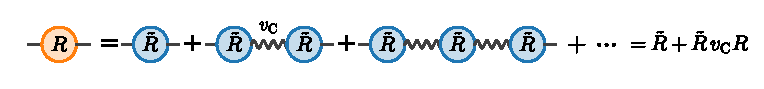
\includegraphics[width=\linewidth]{figures/ch04/fig4_4.pdf}
  \caption{Schematic of the relation between the density response $R$ and its Coulomb-proper part $\tilde R$. Each shaded blob is the proper response of the electrons, which includes every interaction effect except the long-range Coulomb field at the momentum transfer $\vect{q}$. Each wavy line is the Coulomb kernel $v_{\mathrm{C}}(q) = e^2/q^2$, which carries the potential of the charge induced in one blob to the next. Summed, the chain is the geometric series $R = \tilde R + \tilde Rv_{\mathrm{C}}\tilde R + \cdots$, whose closed form is $R = \tilde R + \tilde Rv_{\mathrm{C}}R$. The drawing is a schematic, not a set of Feynman rules.}
  \label{fig:4-series}
\end{figure}

The ratio of the external to the total potential is the dielectric function. From \cref{eq:4.4-phitot,eq:4.4-proper}, $\phi_{\mathrm{ext}} = (1 - v_{\mathrm{C}}\tilde R_{ee})\,\phi_{\mathrm{tot}}$ and $\phi_{\mathrm{tot}} = (1 + v_{\mathrm{C}}R_{ee})\,\phi_{\mathrm{ext}}$. Hence
\begin{equation}
  \varepsilon(\vect{q},\omega) \equiv \frac{\phi_{\mathrm{ext}}}{\phi_{\mathrm{tot}}} = 1 - v_{\mathrm{C}}(q)\,\tilde R_{ee}(\vect{q},\omega), \qquad
  \varepsilon^{-1}(\vect{q},\omega) = 1 + v_{\mathrm{C}}(q)\,R_{ee}(\vect{q},\omega) ,
  \label{eq:4.4-eps}
\end{equation}
and the two forms are each other's inverse by \cref{eq:4.4-dyson}. These are the relations \cref{eq:A.7-eps,eq:A.7-L} stated in \cref{app:A.7}, and the second is Ref.~\cite[Eq.~(5)]{knapen2021dark} in our units. We write $\varepsilon = \varepsilon_1 + \ii\varepsilon_2$. The classical reading is the familiar one. In Heaviside--Lorentz units the external charge is the source of $\vect{D}$ and the total charge the source of $\vect{E}$. For a longitudinal field the potential energies are proportional to the potentials, so $\varepsilon$ is the ratio $D/E$ of the Fourier components, the dielectric function of classical electromagnetism, now for every $\vect{q}$ and $\omega$. It is the longitudinal dielectric function, because a potential produces a field along $\vect{q}$.

The inverse function $\varepsilon^{-1} - 1 = v_{\mathrm{C}}R_{ee}$ is a retarded response, the induced potential per unit external one, and it has every property \cref{sec:4.1,sec:4.3} proved for $R_{ee}$: analyticity in the upper half plane, the Kramers--Kronig relations, and $\Imag\varepsilon^{-1} \le 0$ for $\omega > 0$. The function $\varepsilon - 1$ obeys the Kramers--Kronig relations only because a stable target has no zeros of $\varepsilon$ in the upper half plane (\cref{eq:C.5-KKeps}). The static limit of $\varepsilon^{-1}v_{\mathrm{C}}$ is the statically screened Coulomb interaction: an external point charge, or a second electron held at rest, acts through $v_{\mathrm{C}}(q)/\varepsilon(\vect{q},0)$ rather than $v_{\mathrm{C}}(q)$ (\cref{sec:4.8} uses it in the electron self-energy). At small $q$, $v_{\mathrm{C}}$ grows as $1/q^2$, and this is where screening matters most.

In an insulator the static dielectric function at long wavelength is finite. With the lattice clamped, its value $\varepsilon_\infty = \varepsilon(\vect{q}\to0, \omega\to0)$ is the electronic, or high-frequency, dielectric constant, so called because it is measured at frequencies above those of the lattice vibrations and below the gap; the static constant $\varepsilon_0$ with the lattice included is the subject of \cref{sec:5.5}. For silicon $\varepsilon_\infty = 11.7$~\cite{franta2017temperature}: a static charge in the crystal is screened to a twelfth of its bare strength at distances of many cells. Where $\varepsilon_1$ crosses zero and $\varepsilon_2$ is small, the external potential produces a large total one, and the electrons oscillate collectively. This is the plasmon, a pole of \cref{eq:4.4-dyson} near the real axis, which appears as a peak of $\Imag(-\varepsilon^{-1})$; \cref{sec:4.5} makes it precise.

\subsection{Local fields and the dielectric matrix}

In a crystal a potential at $\vect{q}$ also induces density at $\vect{q} + \vect{G}$ for every reciprocal-lattice vector $\vect{G}$ (\cref{sec:4.1}): the electrons pile up near the atoms and in the bonds, on the scale of the cell, not uniformly. The density and the potentials are then vectors indexed by $\vect{G}$, at a wavevector $\vect{q}$ in the first zone, and the response is a matrix,
\begin{equation}
  R_{\vect{G}\vect{G}'}(\vect{q},\omega) = R_{ab}(\vect{q},\omega)\big|_{O_a = n_e(\vect{q}+\vect{G}),\ O_b = n_e(\vect{q}+\vect{G}')} ,
  \label{eq:4.4-RGG}
\end{equation}
the density response at $\vect{q} + \vect{G}$ to a potential at $\vect{q} + \vect{G}'$, from the Kubo formula of \cref{sec:4.1}. Each Fourier component of the induced density produces its own Hartree potential, $v_{\mathrm{C}}(|\vect{q}+\vect{G}|)\,\delta\nd_{e,\vect{G}}$, and \cref{eq:4.4-phitot,eq:4.4-proper} become matrix equations. The same steps lead to $R = \tilde R + \tilde R\,v_{\mathrm{C}}\,R$, with $v_{\mathrm{C}}$ the diagonal matrix of $v_{\mathrm{C}}(|\vect{q}+\vect{G}|)$, and to the dielectric matrix
\begin{equation}
  \varepsilon_{\vect{G}\vect{G}'}(\vect{q},\omega) = \delta_{\vect{G}\vect{G}'} - v_{\mathrm{C}}(|\vect{q}+\vect{G}|)\,\tilde R_{\vect{G}\vect{G}'}(\vect{q},\omega), \qquad
  \bigl(\varepsilon^{-1}\bigr)_{\vect{G}\vect{G}'} = \delta_{\vect{G}\vect{G}'} + v_{\mathrm{C}}(|\vect{q}+\vect{G}|)\,R_{\vect{G}\vect{G}'} ,
  \label{eq:4.4-epsGG}
\end{equation}
for any proper response $\tilde R$, exact or approximate. That the two matrices are inverses of each other takes one line of matrix algebra (\cref{app:D.7}). This is \cref{eq:A.7-eps}, the unsymmetrized counterpart of the symmetrized longitudinal dielectric matrix of Ref.~\cite[Eqs.~(A5)--(A7)]{knapen2021dark}, which is built with $v_{\mathrm{C}}^{1/2}\tilde Rv_{\mathrm{C}}^{1/2}$ and has the same diagonal elements of the inverse (\cref{app:D.7}).

An experiment with a long-wavelength field sees the average of the total field over a cell. The external field has only the component $\vect{G}' = 0$, and the cell average of the total field is its component $\vect{G} = 0$ (\cref{eq:A.3-periodic}), which is $(\varepsilon^{-1})_{\vect{0}\vect{0}}$ times the external one. The macroscopic dielectric function is therefore
\begin{equation}
  \varepsilon_{\mathrm{mac}}(\vect{q},\omega) = \frac{1}{\bigl(\varepsilon^{-1}\bigr)_{\vect{0}\vect{0}}(\vect{q},\omega)} ,
  \label{eq:4.4-epsmac}
\end{equation}
the inverse of the head of the inverse matrix, not the head $\varepsilon_{\vect{0}\vect{0}}$ itself~\cite{adler1962quantum,wiser1963dielectric}. The head $\varepsilon_{\vect{0}\vect{0}}$ answers a different question: the external potential needed at $\vect{G} = 0$ to produce a total potential that has only a $\vect{G} = 0$ component. No macroscopic external field produces such a total potential in a crystal. The two differ because the macroscopic field drives density at all $\vect{G}$, and the Hartree potentials of these microscopic components feed back on the $\vect{G} = 0$ component. Inverting the matrix in blocks (\cref{eq:C.7-head}) gives the correction explicitly,
\begin{equation*}
  \varepsilon_{\mathrm{mac}} = \varepsilon_{\vect{0}\vect{0}} - \sum_{\vect{G},\vect{G}'\ne0}\varepsilon_{\vect{0}\vect{G}}\,\bigl[(\varepsilon_{\ne0})^{-1}\bigr]_{\vect{G}\vect{G}'}\,\varepsilon_{\vect{G}'\vect{0}} ,
\end{equation*}
with $\varepsilon_{\ne0}$ the block with $\vect{G},\vect{G}' \ne 0$. The sum is the local-field effect: the difference between the response to the average field and the response to the field that the electrons actually feel inside the cell. \Cref{app:D.7} shows that it stays finite as $\vect{q} \to 0$ although single elements of the matrix diverge there, and writes $\varepsilon_{\mathrm{mac}}$ in the equivalent form $1 - v_{\mathrm{C}}(q)\bar R_{\vect{0}\vect{0}}$, with $\bar R$ the response computed with the Coulomb kernel at $\vect{G} = 0$ removed~\cite{onida2002electronic}. In a homogeneous system the off-diagonal elements vanish and $\varepsilon_{\mathrm{mac}} = \varepsilon_{\vect{0}\vect{0}} = \varepsilon$; how large the local-field effects of silicon are in the random-phase approximation is the subject of \cref{sec:4.6}. The macroscopic function is the one measured optically, and $\varepsilon_\infty$ is its static limit at $\vect{q} \to 0$. For a momentum transfer beyond the first zone, $\vect{q} = \vect{q}_r + \vect{G}_q$ as in \cref{eq:3.1-qsplit}, the same reasoning applies at the row and column of $\vect{G}_q$, which is the unreduced indexing of \cref{eq:A.3-unreduced}: $(\varepsilon^{-1})_{00}(\vect{q},\omega)$ means $(\varepsilon^{-1})_{\vect{G}_q\vect{G}_q}(\vect{q}_r,\omega)$.

\subsection{Structure factor and loss function}

The rate needs $S$, and the fluctuation--dissipation theorem \cref{eq:4.2-fdt} ties $S$ to $\Imag R_{ee}$, which \cref{eq:4.4-eps} ties in turn to the inverse dielectric function. Taking the imaginary part of $\varepsilon^{-1} = 1 + v_{\mathrm{C}}R_{ee}$, with $v_{\mathrm{C}}$ real, leads to $\Imag\varepsilon^{-1} = v_{\mathrm{C}}\Imag R_{ee}$, and with $S = -2\Imag R_{ee}/(1 - \ee^{-\beta\omega})$,
\begin{keyresult}[Structure factor and loss function]
\begin{equation}
  S(\vect{q},\omega) = \frac{2q^2}{e^2}\,\frac{L(\vect{q},\omega)}{1 - \ee^{-\beta\omega}} = \frac{q^2}{2\pi\alpha}\,\frac{L(\vect{q},\omega)}{1 - \ee^{-\beta\omega}}, \qquad
  L(\vect{q},\omega) = \Imag\bigl[-\bigl(\varepsilon^{-1}\bigr)_{00}(\vect{q},\omega)\bigr] ,
  \label{eq:4.4-SL}
\end{equation}
for the density response of the electrons with the nuclei clamped. The loss function $L$ is nonnegative for $\omega > 0$, and the rate of any density coupling is fixed by it.
\end{keyresult}
This is \cref{eq:A.7-SL}, Ref.~\cite[Eq.~(6)]{knapen2021dark}, and at $T = 0$ Ref.~\cite[Eqs.~(S.7) and (S.24)]{hochberg2021determining}. In a crystal the derivation goes through element by element. By \cref{eq:4.4-RGG} the diagonal element of $R_{\vect{G}\vect{G}'}(\vect{q}_r,\omega)$ at $\vect{G} = \vect{G}' = \vect{G}_q$ is the density response $R_{ee}(\vect{q},\omega)$ at the unreduced $\vect{q} = \vect{q}_r + \vect{G}_q$, and \cref{eq:4.4-epsGG} relates it to the diagonal element of $\varepsilon^{-1}$ at the same place. The loss function is that element, local fields included, and the relation holds at each vector $\vect{q}$ with no assumption of isotropy. The name comes from the energy loss of fast electrons in thin films, whose spectrum measures $L$ directly; \cref{eq:4.4-dEdx} below makes the connection.

The relation needs weak single scattering, a coupling to the density, and a probe that sees the electrons alone, and each of these fails somewhere. The probe acts once and weakly, so that the golden rule and linear response apply; this is the Born approximation of \cref{sec:2.2}. It couples to the electrons through their density alone, through a potential that depends on their positions, and not through spin or current~\cite{hochberg2021determining}; spin couplings need the spin response of \cref{chap:7}, and velocity-dependent couplings the current response of \cref{chap:8}. Finally, it couples to the electrons only, or the nuclei are clamped.

The last condition separates two kinds of probe. A test charge, a photon or a dark photon, whose coupling to matter is the photon's scaled by the mixing $\zeta$ (\cref{sec:1.4}), acts on the total charge, $n_Z = -n_e + \sum_\kappa Z_\kappa n_\kappa$ of \cref{sec:2.3}. The dielectric function measured with such probes is $\varepsilon^{-1} = 1 + v_{\mathrm{C}}R_{ZZ}$, with the response of the total charge, and its loss function $L$ fixes the total-charge structure factor exactly, $S_{ZZ} = (2q^2/e^2)\,L/(1 - \ee^{-\beta\omega})$. A mediator that couples to electrons but not to nucleons sees $S = S_{ee}$ instead, and the relation \cref{eq:4.4-SL} holds exactly with the electron-channel function $\varepsilon_e^{-1} = 1 + v_{\mathrm{C}}R_{ee}$ and its loss $L_e$ (\cref{app:A.7}). With the nuclei clamped, $n_\kappa$ contributes only static Bragg terms, $R_{ZZ} = R_{ee}$, and $L_e = L$. With moving nuclei the two differ at phonon energies, where the nuclear charge oscillates and the electrons partly follow it (\cref{chap:5}). Optical and electron-energy-loss experiments measure the total-charge $L$. They yield the dark-photon rate exactly at every energy~\cite{hochberg2021determining}, and the rate of an electron-only coupling at energies well above the phonon band, which is where electronic excitations live. The interference between electron and nuclear densities between those two cases is the business of \cref{chap:8}.

For a scalar dielectric function, with the local fields neglected or in a homogeneous system, $L = \varepsilon_2/|\varepsilon|^2$. Since $\varepsilon_2 = -v_{\mathrm{C}}\Imag\tilde R_{ee}$, the absorptive part of the proper response, \cref{eq:4.4-SL} becomes $S = S^{\mathrm{prop}}/|\varepsilon|^2$, where $S^{\mathrm{prop}} = (2q^2/e^2)\,\varepsilon_2/(1 - \ee^{-\beta\omega})$ is the structure factor built from $\tilde R_{ee}$ (\cref{eq:A.7-SL}). The rate is the rate of the proper response, screened by $1/|\varepsilon|^2$. In the random-phase approximation the proper response is the independent-particle one, $S^{\mathrm{prop}} = S^0$ of \cref{eq:4.2-S0}, and the factor $1/|\varepsilon|^2$ is what earlier calculations of the dark-matter--electron rate left out~\cite{knapen2021dark}.

\Cref{fig:4-siloss} shows what the factor does in silicon at $q \to 0$. Absorption, $\varepsilon_2$, is strong between the gap and about \SI{10}{eV}, with peaks at 3.4 and \SI{4.2}{eV} from interband transitions. There, however, $|\varepsilon|$ is large, and the loss function is small: at \SI{3}{eV}, $\varepsilon_2 = 2.4$ but $L = 3.1\times10^{-3}$. The real part $\varepsilon_1$ is negative from \SI{4.2}{eV} and crosses zero again at \SI{16.3}{eV}, where $\varepsilon_2$ has fallen below one. The loss function peaks there, at \SI{16.4}{eV}, with a height of 4.5 and a full width of \SI{3.7}{eV}. This is the plasmon of the valence electrons; how its position relates to the free-electron $\omega_p$ is the subject of \cref{sec:4.5}. For a dark-matter particle, which can deposit at most $qv_{\mathrm{max}}$, the consequence is that the energies it reaches at typical momentum transfers, a few eV, are those where the target absorbs strongly and screens strongly at once.

\begin{figure}[tbp]
  \centering
  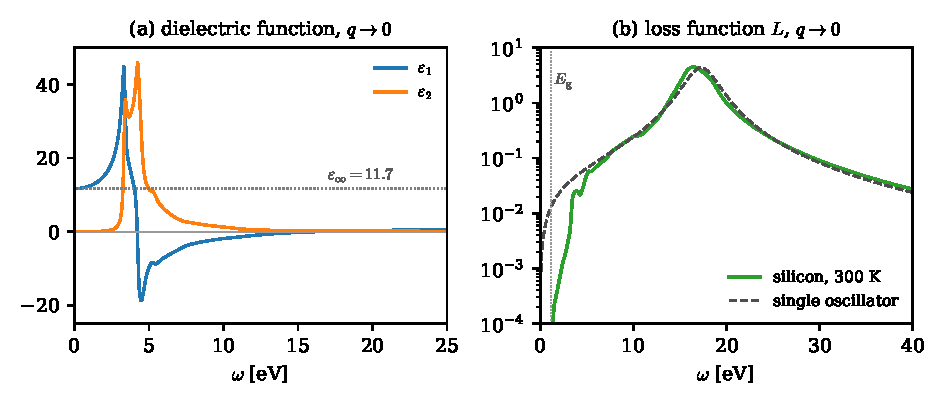
\includegraphics[width=\linewidth]{figures/ch04/fig4_5.pdf}
  \caption{Dielectric function and loss function of crystalline silicon at $q \to 0$ and \SI{300}{K}, from the optical constants of Franta and coworkers, a Kramers--Kronig-consistent dispersion model fitted to ellipsometric and spectrophotometric measurements and tabulated from \SI{4}{meV} to \SI{40}{eV}~\cite{franta2017temperature}. The data are optical, that is transverse; at $q \to 0$ the transverse and longitudinal functions coincide (\cref{eq:4.4-ET}), and $L = \varepsilon_2/|\varepsilon|^2$. (a) $\varepsilon_1$ and $\varepsilon_2$; at low energy $\varepsilon_1 = \varepsilon_\infty = 11.7$ (dotted). The interband peaks of $\varepsilon_2$ lie at 3.4 and \SI{4.2}{eV}, and $\varepsilon_1$ crosses zero upward at \SI{16.3}{eV}. (b) The loss function on a logarithmic scale (solid), with its peak of 4.5 at \SI{16.4}{eV}. Dashed: the single damped oscillator of \cref{we:4-oscillatorL} at $q = 0$, which has the same f-sum and the same $\varepsilon_\infty$, and a damping equal to the measured full width, \SI{3.66}{eV}. Dotted: the room-temperature gap, \SI{1.12}{eV}, to match the data. Below \SI{40}{eV} the tabulated spectrum collects 96 percent of the f-sum of the four valence electrons in $\int\omega\varepsilon_2\,\dd\omega$ and 92 percent in $\int\omega L\,\dd\omega$.}
  \label{fig:4-siloss}
\end{figure}

\subsection{Sum rules for the loss function}

The sum rules of \cref{sec:4.3} carry over. For the f-sum we start from its form at any temperature, $\int_0^\infty\dd\omega\,\omega(1 - \ee^{-\beta\omega})S = \pi\nd_eq^2/m_e$, which folds the negative frequencies onto the positive ones with detailed balance. By \cref{eq:4.4-SL} the factor $(1 - \ee^{-\beta\omega})S$ is $(2q^2/e^2)L$, the temperature drops out, and with $\omega_p^2 = e^2\nd_e/m_e$ from \cref{eq:4.3-wp},
\begin{equation}
  \int_0^\infty\dd\omega\;\omega\,L(\vect{q},\omega) = \frac{\pi}{2}\,\omega_p^2 ,
  \label{eq:4.4-fsumL}
\end{equation}
at every $\vect{q}$ and temperature, with $L$ for the electron channel, or the total one at clamped nuclei. This is \cref{eq:A.7-fsumL} and Ref.~\cite[Eq.~(S.10)]{hochberg2021determining}. With moving nuclei the total-charge $L$ collects in addition the nuclear share of the charge f-sum of \cref{sec:4.3}, $2.73\times10^{-4}$ of the total for silicon.

The absorptive part obeys the same rule. The macroscopic $\varepsilon_2$ is $-v_{\mathrm{C}}(q)\Imag\bar R_{\vect{0}\vect{0}}$ (\cref{app:D.7}), and $\bar R$ is the density response of the electrons with the Coulomb kernel at the single wavevector $\vect{q}$ removed from the Hamiltonian. Removing one Fourier component out of a continuum of them changes the equilibrium state by nothing in the thermodynamic limit (\cref{sec:4.8-removal}), while the double commutator of \cref{sec:4.3} does not involve the interaction at all. The response $\bar R$ therefore has the same f-sum as $R$, and
\begin{equation}
  \int_0^\infty\dd\omega\;\omega\,\varepsilon_2(\vect{q},\omega) = \frac{\pi}{2}\,\omega_p^2 ,
  \label{eq:4.4-fsumeps}
\end{equation}
which \cref{app:C.5} also obtains from the Kramers--Kronig relation for $\varepsilon - 1$ at large frequency. The two functions $\varepsilon_2$ and $L$ distribute the same weight differently: $\varepsilon_2$ puts it at the transition energies, and $L = \varepsilon_2/|\varepsilon|^2$ moves it up to where $|\varepsilon|$ is small, toward the plasmon. Tested on the tabulated silicon data of \cref{fig:4-siloss}, the spectrum below \SI{40}{eV} holds 96 percent of $(\pi/2)\omega_p^2 = \SI{433}{eV^2}$ for the four valence electrons in $\int\omega\varepsilon_2$, and 92 percent in $\int\omega L$, which has more of its weight at high energy. The rest lies above the table, where the valence absorption overlaps that of the core (\cref{we:4-sifsum}).

The inverse moments follow from the Kramers--Kronig relations at $\omega = 0$ (\cref{eq:C.5-screening,eq:C.5-KKeps}). For an insulator at $\vect{q} \to 0$,
\begin{equation}
  \frac{2}{\pi}\int_0^\infty\dd\omega\;\frac{L(\omega)}{\omega} = 1 - \frac{1}{\varepsilon_\infty}, \qquad
  \frac{2}{\pi}\int_0^\infty\dd\omega\;\frac{\varepsilon_2(\omega)}{\omega} = \varepsilon_\infty - 1 .
  \label{eq:4.4-inverse}
\end{equation}
In a metal static screening is perfect at long wavelength, $\varepsilon^{-1} \to 0$, and the first integral becomes $\pi/2$ (\cref{app:C.5}). Weighted by $1/\omega$, these integrals converge much faster than the f-sum: the tabulated data of \cref{fig:4-siloss} return 99.8 percent of $\varepsilon_\infty - 1$ and 97.8 percent of $1 - 1/\varepsilon_\infty$ below \SI{40}{eV}.

Together, the f-sum and the inverse moment already say where the weight of $L$ sits at small $q$. Their ratio defines a mean excitation energy, $\bar E^2 = \int\omega L/\int(L/\omega)$, and
\begin{equation}
  \bar E^2 = \frac{\omega_p^2}{1 - 1/\varepsilon_\infty} .
  \label{eq:4.4-Ebar}
\end{equation}
With $\omega_p = \SI{16.6}{eV}$ for the valence electrons and $\varepsilon_\infty = 11.7$, $\bar E = 16.6/0.956 = \SI{17.4}{eV}$. If the loss spectrum were a single line, it would sit there, more than fifteen times above the gap of \SI{1.17}{eV}. By \cref{eq:4.4-SL}, the same holds for the density fluctuations $S$ at $T = 0$: at long wavelengths the valence electrons respond collectively, at energies $\sim\omega_p$, and not at the gap, a point \cref{sec:4.5} makes precise.

\subsection{Optical conductivity and transverse response}

Light, and a dark photon absorbed at rest, act through a transverse field, not a potential, and what the experiment measures is a current. The induced current density $\vect{J}$ is linear in the total field $\vect{E}$, $\vect{J} = \sigma_{\mathrm{cond}}\vect{E}$, which defines the optical conductivity $\sigma_{\mathrm{cond}}(\omega) = \sigma_1 + \ii\sigma_2$. With fields varying as $\ee^{-\ii\omega t}$ (\cref{app:A.3}), the Amp\`ere--Maxwell law in Heaviside--Lorentz units, $\nabla\times\vect{B} = \vect{J} + \partial_t\vect{E}$, written as $\nabla\times\vect{B} = \partial_t\vect{D}$ with $\vect{D} = \varepsilon\vect{E}$, requires $-\ii\omega\varepsilon = \sigma_{\mathrm{cond}} - \ii\omega$, so
\begin{equation}
  \varepsilon = 1 + \frac{\ii\,\sigma_{\mathrm{cond}}}{\omega}, \qquad \sigma_1 = \omega\,\varepsilon_2, \qquad \sigma_2 = \omega\,(1 - \varepsilon_1) .
  \label{eq:4.4-sigma}
\end{equation}
Texts in Gaussian units write $\varepsilon = 1 + 4\pi\ii\sigma_{\mathrm{cond}}/\omega$ (\cref{app:A.2}). The real part $\sigma_1$ is the dissipative one, and by \cref{eq:4.4-fsumeps} it obeys $\int_0^\infty\dd\omega\,\sigma_1 = (\pi/2)\omega_p^2$, the f-sum rule in its optical form. Written with the loss function, $\sigma_1 = \omega|\varepsilon|^2L$~\cite{hochberg2021determining}. For the absorption of a dark photon, the in-medium photon self-energy of \cref{sec:1.4} is $\Pi_{\mathrm{em}} = \omega^2(1 - \varepsilon^{\mathrm{T}}) = -\ii\omega\sigma_{\mathrm{cond}}$: the wave equation $\omega^2\varepsilon^{\mathrm{T}}\vect{A} = k^2\vect{A}$ for a transverse vector potential in the medium is $(\omega^2 - k^2 - \Pi_{\mathrm{em}})\vect{A} = 0$. Its imaginary part, $-\omega\sigma_1$, sets the absorption rate of \cref{eq:1.4-absorption}.

The function that enters here is the transverse dielectric function $\varepsilon^{\mathrm{T}}$, the response to a field perpendicular to $\vect{q}$, while \cref{eq:4.4-eps} defines the longitudinal one. Both come from one tensor. A vector potential $\vect{A}\,\ee^{\ii\vect{q}\cdot\vect{r}}$ in the gauge with no scalar potential, $\vect{E} = -\partial_t\vect{A} = \ii\omega\vect{A}$, enters the kinetic energy of each electron as $(\vect{p} + e\vect{A})^2/2m_e$. To first order it couples to the paramagnetic current $\vect{j}_e(\vect{q})$ of \cref{eq:4.3-continuity} through $e\vect{A}\cdot\vect{j}_e(\vect{q})$, and it changes the velocity of every electron from $\vect{p}/m_e$ to $(\vect{p} + e\vect{A})/m_e$. The induced particle current per volume therefore has two parts. The diamagnetic part is the density times the added velocity, $\nd_e\,e\vect{A}/m_e$. The paramagnetic part is the Kubo response \cref{eq:4.1-kubo} of $\vect{j}_e$ to the perturbation $O_b\phi_{\mathrm{ext}} = j_e^\beta(\vect{q})\,eA^\beta$, which is $\tilde R^{\alpha\beta}_{jj}\,eA^\beta$, with $\tilde R^{\alpha\beta}_{jj}$ the proper current--current response, proper because $\vect{E}$ is the total field. Together,
\begin{equation*}
  \frac{\delta\langle j_e^\alpha(\vect{q})^\dagger\rangle}{\Vol} + \nd_e\frac{eA^\alpha}{m_e} = e\Bigl[\frac{\nd_e}{m_e}\delta^{\alpha\beta} + \tilde R^{\alpha\beta}_{jj}(\vect{q},\omega)\Bigr]A^\beta .
\end{equation*} Multiplying by the electron charge $-e$ and inserting $\vect{A} = -\ii\vect{E}/\omega$,
\begin{equation*}
  \varepsilon^{\alpha\beta}(\vect{q},\omega) = \delta^{\alpha\beta} - \frac{e^2}{\omega^2}\Bigl[\frac{\nd_e}{m_e}\delta^{\alpha\beta} + \tilde R^{\alpha\beta}_{jj}(\vect{q},\omega)\Bigr] .
\end{equation*}
For free electrons $\tilde R_{jj}$ vanishes at $\vect{q} = 0$, since the total momentum is conserved, and $\varepsilon = 1 - \omega_p^2/\omega^2$. The transverse function is $\varepsilon^{\mathrm{T}} = \hat{\vect{e}}\cdot\varepsilon\cdot\hat{\vect{e}}$ for a unit vector $\hat{\vect{e}} \perp \vect{q}$, and the longitudinal one is $\hat{\vect{q}}\cdot\varepsilon\cdot\hat{\vect{q}}$.

That the longitudinal projection is the $\varepsilon$ of \cref{eq:4.4-eps} follows from the continuity equation \cref{eq:4.3-continuity}, $\partial_tn_e(\vect{q},t) = \ii\vect{q}\cdot\vect{j}_e(\vect{q},t)$. In the Kubo integral for $R_{ee}(\vect{q},\omega)$ we integrate by parts in $t$ twice, using $\omega + \ii0^+$ so that the boundary terms at large $t$ vanish. The first boundary term contains the equal-time commutator of two densities, which is zero. The first integration replaces $n_e(\vect{q},t)^\dagger$ by $-\ii\vect{q}\cdot\vect{j}_e(\vect{q},t)^\dagger$; the second, after moving the time to the other operator by stationarity, replaces $n_e(\vect{q},0)$ by $\ii\vect{q}\cdot\vect{j}_e(\vect{q},0)$ and leaves the boundary term $\langle[\vect{q}\cdot\vect{j}_e^\dagger, n_e]\rangle/\Vol = \nd_eq^2/m_e$, the double commutator of the f-sum rule. The result is a Ward identity, the statement of charge conservation for the response functions,
\begin{equation}
  \omega^2R_{ee}(\vect{q},\omega) = \frac{\nd_eq^2}{m_e} + q_\alpha q_\beta\,R^{\alpha\beta}_{jj}(\vect{q},\omega) ,
  \label{eq:4.4-ward}
\end{equation}
exactly, and the same identity holds for the proper functions, by the argument that gave \cref{eq:4.4-fsumeps}~\cite[Chap.~3]{giuliani2005quantum}. Inserted into the tensor, $\hat{\vect{q}}\cdot\varepsilon\cdot\hat{\vect{q}} = 1 - (e^2/q^2)\tilde R_{ee} = \varepsilon$. As $\vect{q} \to 0$, the proper tensor $\tilde R_{jj}^{\alpha\beta}$ tends to a limit that does not depend on the direction of $\vect{q}$, since the proper response has no long-range Coulomb kernel and so no singularity at $\vect{q} = 0$. Both projections are then taken of the same tensor $\varepsilon^{\alpha\beta}(\omega)$. In a cubic crystal that tensor is a multiple of the unit matrix (\cref{app:C.3}), and
\begin{equation}
  \varepsilon^{\mathrm{T}}(\vect{q},\omega) \to \varepsilon(\vect{q},\omega) \qquad (\vect{q} \to 0) .
  \label{eq:4.4-ET}
\end{equation}
In a crystal of lower symmetry the longitudinal function depends on the direction $\hat{\vect{q}}$ even at $\vect{q} \to 0$, but it is still the projection of the optical tensor. This is why optical data at $q \to 0$ give the longitudinal loss function, as in \cref{fig:4-siloss}, and why the absorption of a dark photon and the scattering of dark matter at small $q$ are governed by the same $\varepsilon_2$. At finite $q$ the two functions separate; for dark-matter scattering, which needs momentum transfers of keV, the longitudinal function is the one that matters.

\subsection{Thomas--Fermi screening}

The simplest proper response is that of a gas of electrons in a static potential that varies slowly in space. Each region of the gas then sits in local equilibrium, with the potential energy $\phi_{\mathrm{tot}}(\vect{r})$ shifting all its levels. The electrochemical potential must be the same everywhere, so the local chemical potential is $\mu_{\mathrm{ch}} - \phi_{\mathrm{tot}}(\vect{r})$, and the density changes by $\delta\nd_e = -(\partial\nd_e/\partial\mu_{\mathrm{ch}})\,\phi_{\mathrm{tot}}$. For the free gas, $\partial\nd_e/\partial\mu_{\mathrm{ch}} = 2\mathcal{N}_{\mathrm{F}}$ at $T = 0$, with $\mathcal{N}_{\mathrm{F}}$ per spin from \cref{eq:2.5-fermi}. The proper response is $\tilde R_{ee}(q, 0) = -2\mathcal{N}_{\mathrm{F}}$, and \cref{eq:4.4-eps} gives
\begin{equation}
  \varepsilon_{\mathrm{TF}}(q) = 1 + \frac{k_{\mathrm{TF}}^2}{q^2}, \qquad
  k_{\mathrm{TF}}^2 = 2e^2\mathcal{N}_{\mathrm{F}} = \frac{4\alpha\,m_ek_{\mathrm{F}}}{\pi} = \frac{3\,\omega_p^2}{v_{\mathrm{F}}^2} ,
  \label{eq:4.4-TF}
\end{equation}
where the last two forms use \cref{eq:2.5-fermi,eq:4.3-wp}. The statically screened interaction is
\begin{equation*}
  \frac{v_{\mathrm{C}}(q)}{\varepsilon_{\mathrm{TF}}(q)} = \frac{e^2}{q^2 + k_{\mathrm{TF}}^2} ,
\end{equation*}
the transform of a Yukawa potential $\alpha\,\ee^{-k_{\mathrm{TF}}r}/r$, the same form as a massive mediator (\cref{eq:1.4-yukawa}) with mass $k_{\mathrm{TF}}$. An impurity charge in a metal is screened within a distance $1/k_{\mathrm{TF}}$. This is the Thomas--Fermi theory of screening, after the semiclassical model of the atom by Thomas and Fermi. Its assumptions are a static potential and a slow variation, $q \ll k_{\mathrm{F}}$, so that the local-equilibrium picture holds; \cref{sec:4.5} recovers \cref{eq:4.4-TF} as the static long-wavelength limit of the Lindhard function and gives the corrections.

\begin{workedexample}{The Thomas--Fermi length of the silicon valence electrons}\label{we:4-tf}
Treat the four valence electrons per atom of silicon as a free gas, $\nd_e = \SI{2.00e23}{cm^{-3}}$, with $k_{\mathrm{F}} = \SI{3.57}{keV}$ and $\mathcal{N}_{\mathrm{F}} = \SI{9.2e7}{eV^2}$ (\cref{sec:2.5}). By \cref{eq:4.4-TF}, $k_{\mathrm{TF}}^2 = 4\alpha m_ek_{\mathrm{F}}/\pi = \SI{1.69e7}{eV^2}$, or $k_{\mathrm{TF}} = \SI{4.12}{keV}$, and a screening length $1/k_{\mathrm{TF}} = \SI{0.48}{\angstrom}$, a fifth of the bond length. At the typical momentum transfer $q_0 = \alpha m_e = \SI{3.73}{keV}$, $\varepsilon_{\mathrm{TF}} = 1 + (4.12/3.73)^2 = 2.22$, and the squared potential, which sets the rate, is reduced by $|\varepsilon_{\mathrm{TF}}|^2 = 4.9$.

The estimate is crude because $k_{\mathrm{TF}}$ is not small against $k_{\mathrm{F}}$ and because silicon is an insulator. With $k_{\mathrm{TF}} = 1.15\,k_{\mathrm{F}}$, the screening happens at the wavevectors where the condition $q \ll k_{\mathrm{F}}$ fails, and the Lindhard function of \cref{sec:4.5} screens less than \cref{eq:4.4-TF} at $q \sim k_{\mathrm{F}}$. In an insulator, moreover, the electrons cannot follow a potential that varies over many cells, and its static screening at long wavelength saturates at $\varepsilon_\infty = 11.7$, while the gas formula diverges. The two descriptions meet where $1 + k_{\mathrm{TF}}^2/q^2 = \varepsilon_\infty$, at $q = k_{\mathrm{TF}}/(\varepsilon_\infty - 1)^{1/2} = \SI{1.26}{keV}$, a length $1/q$ of \SI{1.6}{\angstrom}. As a rough picture, then, silicon screens like a metal at the momentum transfers of a few keV that dark matter typically deposits, and like an insulator with a dielectric constant of 11.7 below about \SI{1}{keV}. Both statements concern the static response; the rate needs $\varepsilon$ at the energy deposited, which is why the computed loss function, not \cref{eq:4.4-TF}, enters the calculations of \cref{chap:10}.
\end{workedexample}

\subsection{Dielectric stopping}

A charged particle crossing a solid slows down by exciting it, and the loss function fixes how fast. Take a particle of charge $Z_1e$, heavy enough that its recoil can be neglected, moving with velocity $\vect{v}$. Its potential energy with an electron is $-Z_1e^2/(4\pi r)$, so $\tilde V(\vect{q}) = -Z_1v_{\mathrm{C}}(q)$, and a momentum transfer $\vect{q}$ deposits $\omega = \vect{q}\cdot\vect{v}$, the energy change $\vect{q}\cdot\vect{v} - q^2/2M_1$ of a particle of mass $M_1 \to \infty$. Weighting each momentum transfer in the rate \cref{eq:4.2-rate} by the energy it deposits gives the energy lost per unit time, and dividing by $v$ the energy lost per unit path. At $T = 0$, with \cref{eq:4.4-SL} and $|\tilde V|^2 = Z_1^2e^4/q^4$,
\begin{equation*}
  -\frac{\dd E}{\dd x} = \frac{1}{v}\int\frac{\dd^3q}{(2\pi)^3}\,\frac{Z_1^2e^4}{q^4}\,\frac{2q^2}{e^2}\,\omega\,L(\vect{q},\omega)\Big|_{\omega = \vect{q}\cdot\vect{v}} .
\end{equation*}
For an isotropic $L$ we use polar coordinates about $\vect{v}$, $\dd^3q = 2\pi q^2\dd q\,\dd u$ with $u$ the cosine of the angle, and change variables from $u$ to $\omega = quv$, $\dd u = \dd\omega/(qv)$. Only $\omega > 0$ contributes at $T = 0$, and
\begin{equation}
  -\frac{\dd E}{\dd x} = \frac{Z_1^2e^2}{2\pi^2v^2}\int_0^\infty\frac{\dd q}{q}\int_0^{qv}\dd\omega\;\omega\,L(q,\omega) = \frac{2Z_1^2\alpha}{\pi v^2}\int_0^\infty\frac{\dd q}{q}\int_0^{qv}\dd\omega\;\omega\,L(q,\omega) .
  \label{eq:4.4-dEdx}
\end{equation}
This is Lindhard's dielectric formula for the stopping power~\cite{lindhard1954properties}, in Heaviside--Lorentz units. The fast and the slow limits show what it contains. For a fast particle, $qv$ reaches beyond the whole loss spectrum at all but the smallest $q$, and the inner integral is the f-sum $(\pi/2)\omega_p^2$. The stopping power is $Z_1^2\alpha\omega_p^2/v^2$ times a logarithm of the range of $q$ that contributes: the Bethe formula, set by the electron density alone. For a slow particle, $qv$ stays below the main peak, and the inner integral samples only the low-energy side of $L$, which the sum rules do not fix. The same is true of a dark-matter particle, which is a slow probe in exactly this sense.

\begin{workedexample}{A single damped oscillator}\label{we:4-oscillatorL}
The simplest loss function consistent with the f-sum and with $\varepsilon_\infty$ puts all the weight in one damped oscillator. Write
\begin{equation*}
  \varepsilon^{-1}(q,\omega) = 1 + \frac{\omega_p^2}{\omega^2 - \omega_{\mathrm{res}}^2 + \ii\varGamma_{\mathrm{w}}\omega}, \qquad
  \omega_{\mathrm{res}}(q)^2 = \bar E^2 + \Bigl(\frac{q^2}{2m_e}\Bigr)^2 ,
\end{equation*}
with a damping rate $\varGamma_{\mathrm{w}}$. The resonance frequency moves from $\bar E$ at small $q$ to the free recoil energy $q^2/2m_e$ at large $q$; this dispersion is our modeling choice, made so that the large-$q$ limit has the free-recoil center that \cref{sec:4.3} requires. The function $\varepsilon^{-1} - 1$ has the form of the damped-oscillator response of \cref{we:4-oscillator}, with $\omega_p^2$ for $2\lambda_{\mathrm{osc}}^2\omega_0$ and $\omega_{\mathrm{res}}$ for $\omega_0$. It is causal, and its imaginary part is
\begin{equation*}
  L(q,\omega) = \frac{\omega_p^2\,\varGamma_{\mathrm{w}}\,\omega}{(\omega^2 - \omega_{\mathrm{res}}^2)^2 + \varGamma_{\mathrm{w}}^2\omega^2} .
\end{equation*}
Integrating, $\int_0^\infty\omega L\,\dd\omega = (\pi/2)\omega_p^2$ for any $\varGamma_{\mathrm{w}}$ and $q$, the f-sum \cref{eq:4.4-fsumL}, and $\int_0^\infty(L/\omega)\,\dd\omega = (\pi/2)\omega_p^2/\omega_{\mathrm{res}}^2$. At $q \to 0$ the inverse moment \cref{eq:4.4-inverse} then requires $1 - 1/\varepsilon_\infty = \omega_p^2/\bar E^2$, which is \cref{eq:4.4-Ebar}: the single oscillator that satisfies both sum rules has its loss peak at the mean excitation energy, $\bar E = \SI{17.4}{eV}$ for silicon. Inverting, $\varepsilon$ itself has its resonance lower, at $(\bar E^2 - \omega_p^2)^{1/2} = \bar E/\varepsilon_\infty^{1/2} = \SI{5.08}{eV}$, and $\varepsilon(0,0) = 11.7$. We take $\varGamma_{\mathrm{w}} = \SI{3.66}{eV}$, the measured full width of the silicon loss peak, which sets the peak height $\omega_p^2/(\varGamma_{\mathrm{w}}\bar E) = 4.34$ against the measured 4.5 (\cref{fig:4-siloss}b).

By \cref{eq:4.4-SL}, the structure factor at $T = 0$ is
\begin{equation*}
  S(q,\omega) = \frac{q^2}{2\pi\alpha}\,\frac{\omega_p^2\,\varGamma_{\mathrm{w}}\,\omega}{(\omega^2 - \omega_{\mathrm{res}}^2)^2 + \varGamma_{\mathrm{w}}^2\omega^2} ,
\end{equation*}
and its first moment is $(q^2/2\pi\alpha)(\pi/2)\omega_p^2 = \pi\nd_eq^2/m_e$, the f-sum \cref{eq:4.3-fsum}. As $\varGamma_{\mathrm{w}} \to 0$, the weight collapses onto $\omega = \omega_{\mathrm{res}}$ with $\int\dd\omega\,S = \pi\nd_eq^2/(m_e\omega_{\mathrm{res}})$, and by \cref{eq:4.2-static} $S^{\mathrm{st}} = q^2/(2m_e\omega_{\mathrm{res}})$: the density fluctuations vanish as $q^2$ at small $q$, below the bound $q^2/(2m_e\Eg)$ of \cref{sec:4.3} since $\omega_{\mathrm{res}} > \Eg$.

For the stopping power of a slow particle, take $qv \ll \omega_{\mathrm{res}}$ at every $q$. Since $\omega_{\mathrm{res}}/q$ is smallest, $(\bar E/m_e)^{1/2} = 5.8\times10^{-3}$, at $q = (2m_e\bar E)^{1/2} = \SI{4.2}{keV}$, this means $v \ll 5.8\times10^{-3}$. Then $L \simeq \omega_p^2\varGamma_{\mathrm{w}}\omega/\omega_{\mathrm{res}}^4$ on the whole range of the inner integral of \cref{eq:4.4-dEdx}, which becomes $\omega_p^2\varGamma_{\mathrm{w}}q^3v^3/(3\omega_{\mathrm{res}}^4)$. With $q = (2m_e\bar E)^{1/2}x$, the remaining integral is $\int_0^\infty q^2\dd q/\omega_{\mathrm{res}}^4 = (2m_e\bar E)^{3/2}\bar E^{-4}\int_0^\infty x^2\dd x/(1 + x^4)^2$, and the last integral is $\pi/(8\sqrt2)$. Altogether
\begin{equation*}
  -\frac{\dd E}{\dd x} \simeq \frac{Z_1^2\,\alpha\,\varGamma_{\mathrm{w}}\,\omega_p^2\,m_e^{3/2}}{6\,\bar E^{5/2}}\;v .
\end{equation*}
The slow particle feels a friction proportional to its speed, with a coefficient set by the damping. For silicon's numbers and $Z_1 = 1$ it is \SI{0.18}{eV/\angstrom} at $v = 10^{-3}$; the full integral \cref{eq:4.4-dEdx} gives \SI{0.186}{eV/\angstrom}, 3 percent more, and 22 percent more at $v_{\mathrm{max}} = 2.65\times10^{-3}$, where the condition $v \ll 5.8\times10^{-3}$ is only marginal.

The coefficient tests only the tail of the model. The energies that matter are up to $qv \approx \SI{4}{eV}$ at the dominant $q \approx \SI{4}{keV}$, and there the oscillator and silicon disagree badly: at \SI{3}{eV} the model has $L = 0.035$, eleven times the measured value, and it has weight below the gap, where silicon has none (\cref{fig:4-siloss}b). Both loss functions satisfy the f-sum and give the same $\varepsilon_\infty$. The sum rules fix the main peak, while slow particles, and dark matter, sample the low-energy side of $L$, which only a calculation or a measurement of the actual material can supply.
\end{workedexample}
